\chapter{System Interaction Diagrams}

% This chapter requires a good 1-2 pages
% prefacing the way systems will behave
% and introducing the types of diagrams
% that will be shown.

\section{Introduction}
Following is an analysis of the interactions of the two most important internal subsystems in our system as identified in our domain model, the financial data retrieval subsystem and the asynchronous processing subsystem. The interaction diagrams included clearly describe the interactions that occur within each of these subsystems. They elaborate upon the mechanics behind our use cases, but do not necessarily correspond to them one-to-one. This is because several of our use cases are completely facilitated through the browser and controller to generate views for the users, and as such it would not be interesting or worthwhile to explore the internal interactions. The following analysis clearly describes how market orders are placed and processes, how information is retrieved from Yahoo! Finance, and how we manage asynchronous processes (i.e. a queue) in order to process market orders and enact our mailer system.
 
\section{Financial Data Retrieval Subsystem}

\subsection{Enter the Capital Games Financial Adaptor}

For the querying and retrieval of real time and historical financial data and stock quotes in a form that is both familiar and friendly to players of Capital Games, we will utilize the {\textit{\textbf{Yahoo! Finance}}} Application Programming Interface (API), which allows for easy access of {\textit{\textbf{Yahoo! Finance}}} stock data via data served via URLs that our system can retrieve, parse, and then translate for the use of Capital Games’ fantasy leagues platform. Since we will be drawing data from {\textit{\textbf{Yahoo! Finance}}}, it will be represented as external to the system of Capital Games. Internal to our system, however, will be the financial adaptor module that will automatically handle data retrieval from {\textit{\textbf{Yahoo! Finance}}} based on user queries.  

We chose this route over either option of having financial data querying and retrieval built-in to our system or taken from any other API because attempting to construct a built-in, live stock-querying system within Capital Games itself would have been both expensive and impractical --- much akin to reinventing the wheel --- and because {\textit{\textbf{Yahoo! Finance}}} has proven itself as stable and reliable versus other available APIs. Thus, this section will explain our intended financial adaptor module for seamlessly delivering {\textit{\textbf{Yahoo! Finance}}} data for use within Capital Games.

Essentially, by us deploying the a financial adaptor module into Capital Games, users will be able to easily search for stock data within our website and have it near-instantly displayed on the web page they are viewing without the user even being cognizant of all the work being done in the background via our financial adaptor module existing in our server. The financial adaptor module will have all the functionality for making requests for data from {\textit{\textbf{Yahoo! Finance}}} based on user input and will actively draw and translate the raw data from {\textit{\textbf{Yahoo! Finance}}} into a form that can be delivered within our own views ergo the data will be displayed on our web pages.

One consideration we need to take from our end for the building of our financial data is validating user queries for stock symbols. In other words, what would happen in the case that a user attempts to query a stock symbol, company name, industry, or sector that does not exist? To resolve such issues, our adaptor will also draw from our own database built into the website that keeps an updated list of valid stock symbols and names that is drawn from a source similar to {\textit{\textbf{Yahoo! Finance}}}, {\textit{EODData}}. We are using {\textit{EODData}} to supplement our use of the {\textit{\textbf{Yahoo! Finance}}} API as {\textit{EODData}} offers easy retrieval of all stock symbols and names in a method that is similar to {\textit{\textbf{Yahoo! Finance}}}. {\textit{\textbf{Yahoo! Finance}}} unfortunately does not offer that particular feature, so we will be using {\textit{EODData}} as a supplement to that, in that respect. We will essentially update our database via {\textit{EODData}} and our financial adaptor module at each market opening and closure to account for any mergers, acquisitions, or any other major changes involving companies in the stock market.

Once user queries are validated by our financial adaptor module, our financial adaptor module will then parse the user query into a URL format that will allow for the retrieval of data via {\textit{\textbf{Yahoo! Finance}}}. Upon completing this, the URL will then be passed through our financial adaptor to {\textit{\textbf{Yahoo! Finance}}}, from which data will be returned to our financial adaptor module via a comma-separated values format (.csv, a container for easily passing volumes of data), which our financial adaptor will then translate into an arrangement that our views can utilize to deliver to the content to the webpage the user made the query from.  From there, the user can then view the data and choose whether they would like to interact with the queried stock within Capital Games.

To elaborate on the technical specifications of our financial adaptor, the rest of this section will incorporate and explain interaction diagrams of methods used by our financial adaptor, illustrating the process I summarized regarding how our financial adaptor will go through interacting with {\textit{\textbf{Yahoo! Finance}}}, {\textit{EODData}}, and the Capital Games platform.

\subsection{Financial Adaptor Interaction Diagrams}

\begin{figure}
\centering
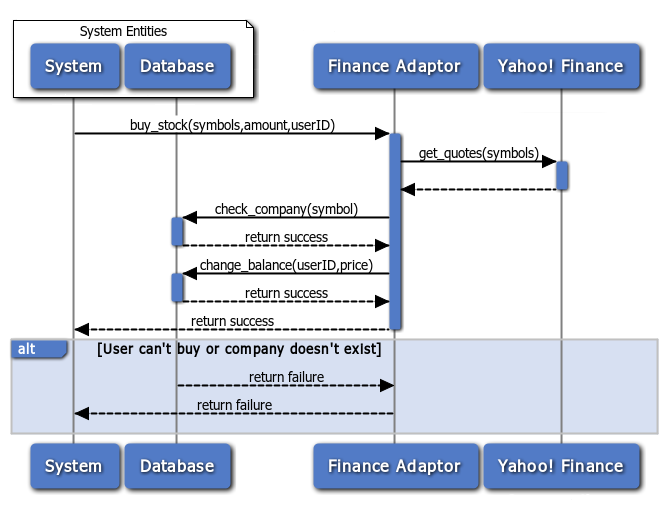
\includegraphics[width=5.5in]{./Diagrams/InteractionDiagrams/buyingstock.png}
\caption{When a user buys a stock, the browser will inform the system of the transaction so that it can be approved. The system passes over the process to the finance adaptor who will check the current price from Yahoo! Finance, check if the company is accepting trades from the database, and check if the user is able to afford the purchase from the database. If all goes well, the transaction will be recorded in the database and the balance will be changed. After all that is complete, the transaction will marked as a success and the system will be notified.}
\end{figure}

\begin{figure}
\centering
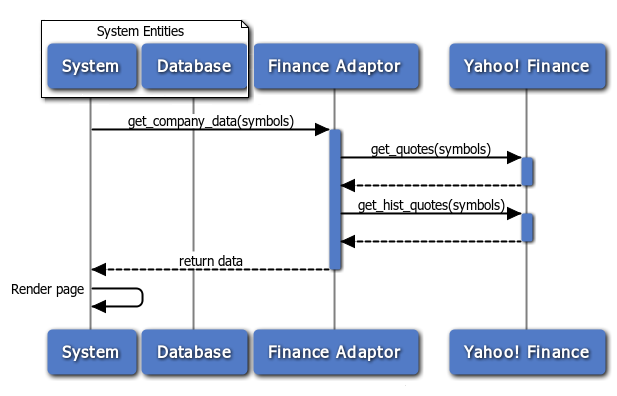
\includegraphics[width=5.5in]{./Diagrams/InteractionDiagrams/rendercompanypage.png}
\caption{When a user wants to view a company page, the company data must be loaded from our finance API. Once the process is passed to the finance adaptor, the quotes and the historical quotes will be pulled from Yahoo! Finance and brought back to the system, who will prepare the page for the user.}
\end{figure}

\begin{figure}
\centering
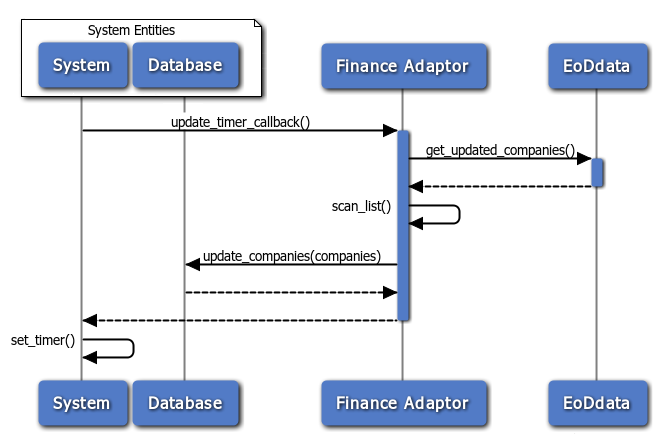
\includegraphics[width=5.5in]{./Diagrams/InteractionDiagrams/updatingdatabase.png}
\caption{We need to keep a local copy of the current companies in our database so we can do rapid processes sing of all of the companies. In order to do this, there will be a timer that is set to update the database every once in a while. When the timer goes off, the system will pass the process onto the finance adaptor. The finance adaptor will then call data from EODData, who knows all of the current companies in the stock market. The finance adaptor will then scan the data for any new/deleted companies and change the database accordingly. After this is complete, the timer will start again so this process can loop.}
\end{figure}

\clearpage
\section{Asynchronous Processing Subsystem}

\subsection{Introduction}

One of Capital Games' primary requirements is to have an asynchronous processing subsystem. This requirement exists both due to the nature of our system, which involves events conditionally occurring at certain time intervals, and the pursuit to build a scalable product. In an attempt to build a system that most closely represents the real stock market, the decision was made to have a pending order queuing system which processes orders at 5 minute intervals. Many orders are processed directly, however some such as short sales and limit orders have conditions associated with them which determine when exactly they are processed. In addition, as the system involves sending summarized reports of player performance metrics at certain time intervals an asynchronous, non-event driven subsystem is highly necessary.\\

\subsection{Nature of the Subsystem}

The asynchronous processing subsystem features three primary components. First, the ability to spawn multiple, independent processes to handle the different kinds of asynchronous tasks. Second, the ability to handle arbitrary object types. And finally, the ability to queue tasks that are waiting to be processed. This is why the Resque Background Process Library built in Ruby was an ideal pick. It allows for the creation of customizable background processes known as "workers". Each worker processes a unique queue. Moreover, each queue can have objects of vastly different types, as long as they implement the function "perform". This is very intuitive as it allows each object to posses the code which acts on it. Lastly, it implements a very smart technique of only storing references to objects in the queue as opposed to the objects themselves so that outdated objects are never processed. This forces the worker to request the most recent version of the object from the DB when it starts being processed. Of course this comes at the slight expense of higher load on the DB when a worker is not sleeping. It is possible that this subsystem will be expanded to incorporate caching techniques. However, they are currently not a requirement. Finally, the queues are stored in RAM for the fastest possible performance. Nevertheless, queues are persisted in JSON encoded flat files to ensure redundancy.\\

\subsection{Structural Model}

\begin{figure}
\centering
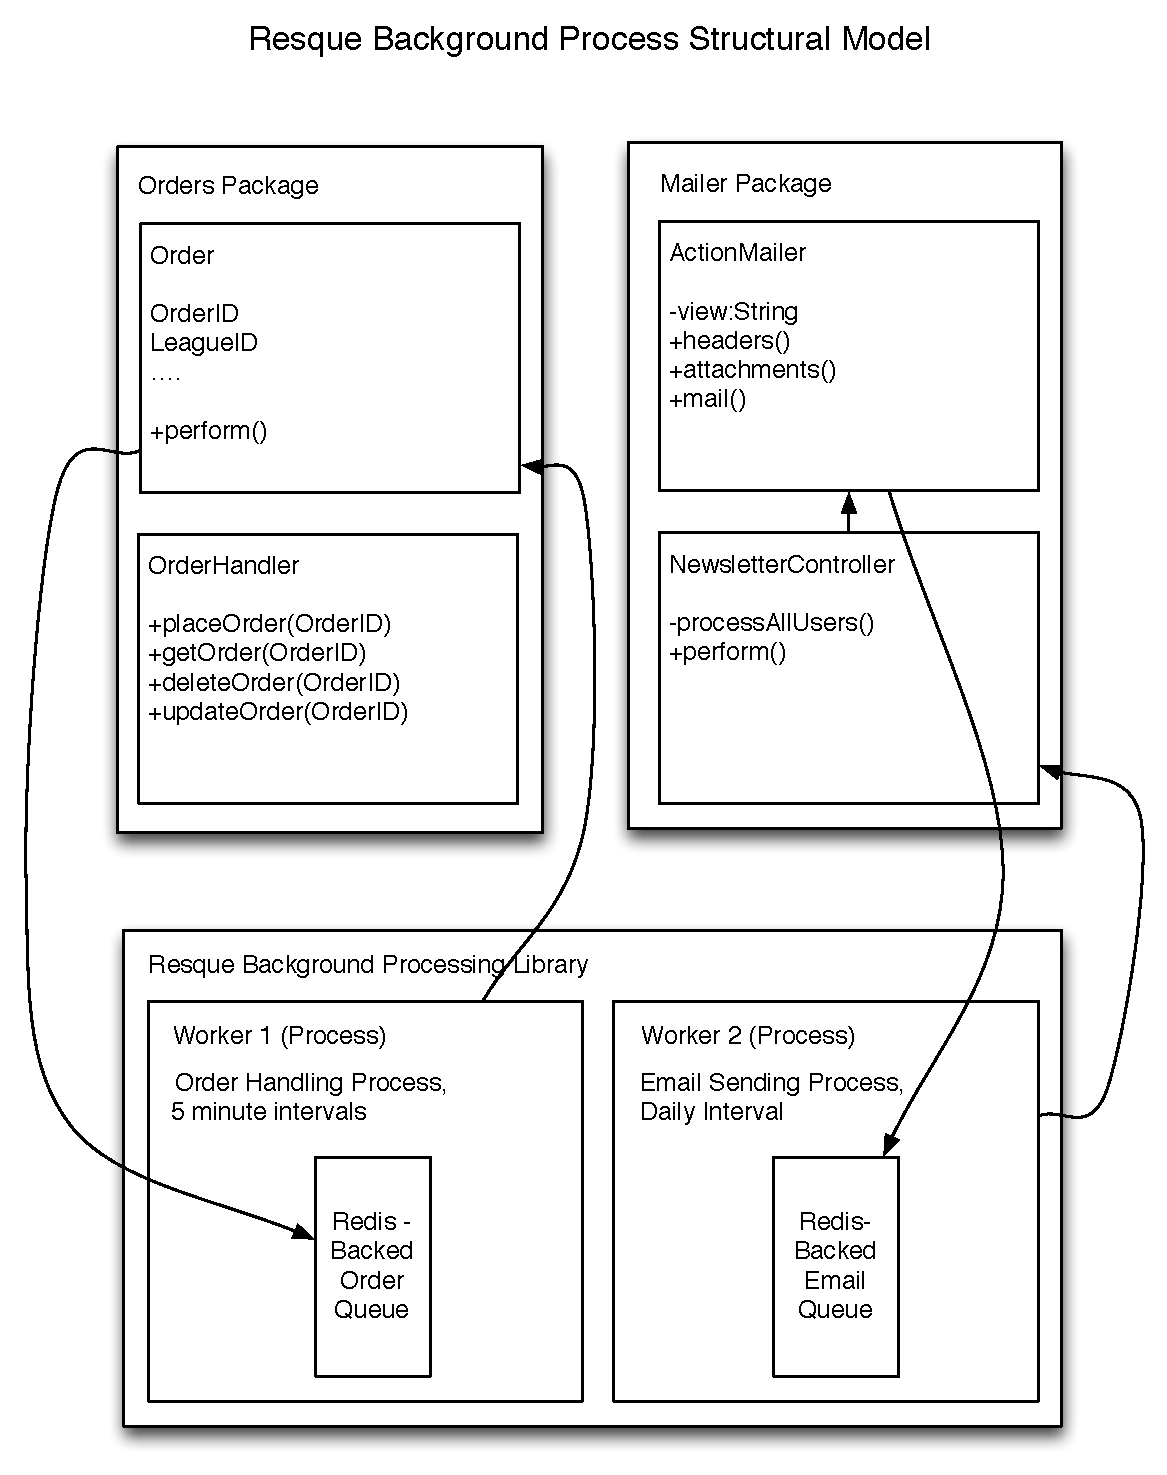
\includegraphics[width=5.5in]{./Diagrams/ComponentModels/BackgroundProcessStructuralModel.pdf}
\caption{The structural model depicts the overall structure of this subsystem. Namely, the Resque Library and two packages or modules which each are responsible for one kind of task. On the left, the orders package displays a relevant subset of all classes that pertain to placing and processing orders. As previously mentioned, the Order object itself implements the perform method. Therefore, it knows how to process its data when it get gets placed in worker 1's queue. While the OrderHandler class isn't directly involved in the asynchronous processing of orders, it is still relevant in this scope and therefore included in the diagram. It is ultimately the class responsible for placing the order object on the queue when an order is placed. Similarly, the mailer package is depicted with a subset of classes which aggregate data about user performance and send out periodic summarizations of performance metrics to all users on the site. Worker 2 is dedicated to processing email related tasks daily. In this case, the architecture is slightly different as the worker doesn't directly call perform on each ActionMailer object, but instead on a NewsletterController which populates the worker's queue with customized ActionMailer Objects.}
\end{figure}

\subsection{Interaction Diagrams}

There are two interaction diagrams displayed below, each associated with one worker. Due to the inherent background nature of this subsystem, there are relatively few actors involved in this subsystem.\\

\begin{figure}
\centering
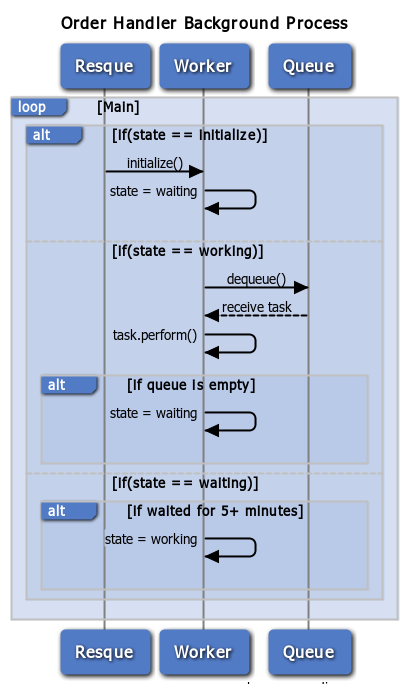
\includegraphics[width=5.5in]{./Diagrams/ComponentModels/stateMachineDiagrams/Worker1/worker1.png}
\caption{The interaction diagram above is roughly divided into two areas, when the process is working and when it is sleeping. This portrays the typical polling behavior of such a background running process. After initialization, when the worker wakes up it attempts to dequeue all objects and call the "perform" method on the object. Since the actual nature of the "perform" method is unique to every object, it is not depicted in this diagram. It is relevant to mention that this individualized execution design allows conditional orders to be processed very easily since the object has all the information needed to make the decision of whether to process at its disposal. Once the queue becomes empty again, the process goes back to sleep. This occurs continually after the spawning of the process.}
\end{figure}

\begin{figure}
\centering
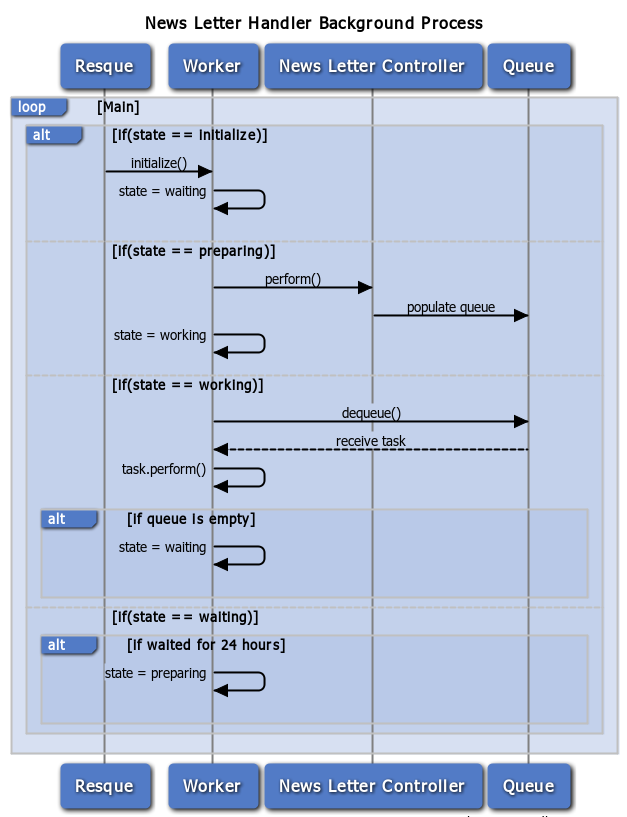
\includegraphics[width=5.5in]{./Diagrams/ComponentModels/stateMachineDiagrams/Worker2/worker2.png}
\caption{Worker 2 behaves a bit differently than worker 1 which results in having an additional state. This "prepare" state is when all the customizing of user-specific emails is done. Afterwards, the process enters the working state where it attempts to fire off all customized emails which were placed onto the queue during the "prepare" state. As in the previous diagram, the diagram incorporates the base case when the worker's queue has been emptied and when the process is sleeping.}
\end{figure}

% Alright, this section requires a solid
% 2-3 pages explaining EVERYTHING LIKE 
% I'M FIVE YEARS OLD. You can't just be like
% "this is how you subsystem". That's what 
% Caggiano does and it's not good enough.
% You need to be like Yates and explain
% everything about the system before you explain
% how to use it. You should explain what a queue
% is, why we chose it (it was the best way to scale
% our load and handle conditional orders), how it's used,
% in what format things are requested and returned
% Then explain how Resque/worker threads abstracts that.
% Then explain the types of methods/classes/jobs you
% created and why they were created. LIKE I'M FIVE!!!
% Then explain how the application interfaces with 
% the subsystem and why I don't need to know your
% subsystem inside and out in order to call into it.
% ONLY THEN can you include diagrams. AND THEN 
% EXPLAIN THEM. People care more about the how and why
% than the what, because from one they should be able
% to intuit the other. 
